\documentclass[11pt]{article}

\usepackage{graphicx}% Include figure files
\usepackage{dcolumn}% Align table columns on decimal point
\usepackage{bm}% bold math
%\usepackage{hyperref}% add hypertext capabilities
%\usepackage[mathlines]{lineno}% Enable numbering of text and display math
%\linenumbers\relax % Commence numbering lines

%\usepackage[showframe,%Uncomment any one of the following lines to test
%%scale=0.7, marginratio={1:1, 2:3}, ignoreall,% default settings
%%text={7in,10in},centering,
%%margin=1.5in,
%%total={6.5in,8.75in}, top=1.2in, left=0.9in, includefoot,
%%height=10in,a5paper,hmargin={3cm,0.8in},
%]{geometry}

\usepackage{longtable}
\usepackage{lipsum}
\usepackage{color}
\usepackage{amsmath}
\usepackage{amssymb}
\usepackage{caption}
\usepackage{subcaption}
\usepackage{hyperref}
\hypersetup{
    colorlinks=true,
    linkcolor=blue,
    filecolor=magenta,      
    urlcolor=cyan,
}

\newcommand{\comment}[1]{}

\setlength{\marginparwidth}{0.75in}
\newcommand{\MarginPar}[1]{\marginpar{%
\vskip-\baselineskip %raise the marginpar a bit
\raggedright\tiny\sffamily
\hrule\smallskip{\color{red}#1}\par\smallskip\hrule}}



\newcommand{\HeatFlux}{\boldsymbol{\mathcal{Q}}}
\newcommand{\SpeciesFlux}{\boldsymbol{\mathcal{F}}}
\newcommand{\SpeciesFluxB}{\bar{\boldsymbol{\mathcal{F}}}}
\newcommand{\StressTensor}{\boldsymbol{\Pi}}
\newcommand{\ShearViscosity}{\eta}
\newcommand{\BulkViscosity}{\kappa}
\newcommand{\ThermalConductivity}{\lambda}
\newcommand{\EntropyProduction}{\mathfrak{v}}
\newcommand{\OnsagerMatrix}{\boldsymbol{\mathfrak{L}}}
\newcommand{\OnsagerMatrixB}{\bar{\boldsymbol{\mathfrak{L}}}}
\newcommand{\OnesVector}{\mathbf{u}}
\newcommand{\ChemicalSpeciesLabel}{\mathfrak{M}}
\newcommand{\StochioPM}{\nu}

\newcommand{\mbar}{\overline{m}}
\newcommand{\Jbar}{\bar{\mathbf{J}}}
\newcommand{\Xbar}{\bar{\mathbf{X}}}
\newcommand{\Lbar}{\bar{\mathbf{L}}}
\newcommand{\Bbar}{\bar{\mathbf{B}}}
\newcommand{\Wbar}{\bar{\mathcal{Z}}}
\newcommand{\Wcbar}{\bar{\mathcal{W}}}
\newcommand{\Bcbar}{\bar{\mathcal{B}}}
\newcommand{\lbar}{\bar{\mathbf{l}}}
\newcommand{\xibar}{\bar{\xi}}
\newcommand{\DonevDiffusion}{{D}}
\newcommand{\half}{\frac{1}{2}}

\begin{document}
\begin{center}
{\bf
Multicomponent reacting compressible Navier Stokes for nonideal gases
}

\vspace{\baselineskip}
John B. Bell \\
Alejandro Garcia \\
Ray Grout \\
Emmanuel Motheau \\
Andrew Nonaka \\
Shashank Yellapantula

\vspace{\baselineskip}
April 19, 2017
\end{center}

\section{TODO: what we need to integrate compressible flow equations}



Guiding principles:
\begin{itemize}
    \item For convenience in the code, they need to be in terms of specific quantities. (Here $\tau$ is specific volume.)
    \item We want to consider cubic equations of state, either SRK or PR. 
    \item We need to have allow for a
        fairly general (up to thermodynamic stability) mixing rule for attractive ($a_m$) and repulsive ($b_m$)
        terms. 
    \item Pressure determines thermodynamics up to a function of temperature.  
        We assume at low pressure (or low density) we approach ideal gas behavior.  That then specifies
        the full thermodynamics of the system.
    \item We compute basic thermodynamic quantities using difference of nonideal pressure and ideal pressure.
    \item Departures can be written in terms of integrals from a reference state (the way Giovangigli does it or compressibility factors)
        From these relations one can compute $e_m$, $s_m$, and $h_m$ where the $m$ subscript denotes the mixture.
        The integrals for SRK are easy when $\tau > b_m$.  PR integrals are uglier.  
\end{itemize}

A list of specifics:
\begin{itemize}
\item Evaluate $p$ given $\rho$, $T$ and $Y_k$. This implicitly involves whatever mixing rules are used to
    evaluate repulsion and attraction terms in cubic EOS \ref{sec:eos}
\item Evaluate sound speed, basically $\partial ln(p)/ \partial ln(\rho)$ at constant entropy and $Y_k$. This
can be expressed in terms of other derivatives. Please see Sec.~\ref{sec:SpeedofSound}. 
\item Need matrix of diffusion coefficients $\mathcal{D}$.  This typically requires binary diffusion coefficients and may involve high density corrections
\item The matrix $\Gamma$ that represents nonideal chemical potential effect on transport
\item The vector of $\theta$'s (or $\phi$'s) that represent volume fractions in barodiffusion
\item Need vector of rescaled thermal diffusion ratios $\tilde{\chi}$ (if you want Soret and Dufour)
\item Thermal conductivity $\lambda$ and viscosity coefficients $\eta$ and $\kappa$
\item The species enthalpies $h_k$ that are need to form energy diffusive flux. Please see Sec.~\ref{sec:PartialEnthalpies}. 
\item The species chemical potentials that are needed for chemistry
\item A specification of chmical rates
\item One probably needs specific heats, at least to compute thermal diffusion time step limit. Please see Eq.~\ref{eq:CpRelation}
\end{itemize}

See John's summary in Secion \ref{sec:john_summ}



\section{Equations}

As a prelude, much of the later parts of this that are specific to SRK equation of state are taken from 
paper by Giovangigli and collaborators \cite{giovangigli_CTM:2011,giovangigli:2012}.

The continuity, species, momentum and energy equations are:
\begin{equation}
\frac{\partial }{\partial t} \left( \rho \right)  + { \nabla} \cdot \left( \rho { u} \right) = 0,
\label{eqn:cont}
\end{equation}
\begin{equation}
\frac{\partial }{\partial t} \left( \rho Y \right)  + { \nabla} \cdot \left( \rho { u} Y \right) + { \nabla} \cdot
\SpeciesFlux
=  \omega 
\label{eqn:spec}
\end{equation}
\begin{equation}
\frac{\partial }{\partial t} \left( \rho { u} \right)  + { \nabla} \cdot \left( \rho { u \otimes u } \right) + { \nabla} p + {\nabla} \cdot   \StressTensor = 0,
\label{eqn:mom}
\end{equation}
\begin{equation}
\frac{\partial }{\partial t} \left( \rho E \right)  + { \nabla} \cdot \left( \rho { u} E + p { u}  \right) + { \nabla} \cdot  { \HeatFlux}  + \nabla \cdot (\StressTensor u)
\label{eqn:energy}
\end{equation}
where $\rho$, ${u}$ and $p$ denote the density, velocity vector and pressure, respectively, of the mixture.
$E = e + \half u^T u$ is the total energy with internal energy $e$.
The mass fraction of the $k$-th species is given by $Y_k$, and is denoted in vector form as $Y$.
The different species in the gaseous mixture are assumed to be in thermal equilibrium,
that is, at a common temperature, $T$.

In the momentum equation, the tensor $\StressTensor$ is the viscous stress and, under the Newtonian assumption, is given by:
\begin{equation}
\StressTensor = \eta ( \nabla u + ( \nabla u )^T) + ( \kappa - \frac{2}{3} \eta) \mathbf{I} \nabla \cdot u
\end{equation}

The formulation of the multi-species stochastic diffusion and heat fluxes is complicated by the couplings among the species fluxes (cross-diffusion effects) and by the thermal diffusion contribution (Soret and Dufour effects).
The starting point for determining these fluxes
is the entropy production for a mixture, as formulated by de Groot and Mazur~\cite{DM_63} and by Kuiken~\cite{NewIrrevThermoBook},
which establishes the form of the thermodynamic forces and fluxes.
The entropy production also has a contribution due to the stress tensor, however,
due to the Curie symmetry principle \cite{DM_63}, fluxes and thermodynamic forces of different tensorial
character do not couple.

%Following Eqn. (IV.13) in De Groot and Mazur,
The entropy production for a
multi-component mixture at rest, in the absence of external forces~\footnote{This contribution
is also zero if the external specific force
acting on each species is constant, as with a constant gravitational acceleration.} and chemistry,
is given by \cite{DM_63}:
%
\begin{eqnarray}
\EntropyProduction &=&
-\frac{1}{T^2} \HeatFlux' \cdot \nabla T
- \frac{1}{T} \sum_{i=1}^{N_s} \SpeciesFlux_i \cdot \nabla_T \mu_i \\
&=& -\frac{1}{T^2} \HeatFlux' \cdot \nabla T
- \frac{1}{T} \sum_{i=1}^{N_s-1} \SpeciesFlux_i \cdot \nabla_T \left(\mu_i - \mu_{N_s} \right ),
\label{eq:dGM1}
\end{eqnarray}
%
where $\mu_i$ is the chemical potential per unit mass of species $i$ and
\begin{equation}
\HeatFlux' = \HeatFlux - \sum_{k=1}^{N_s} h_k \SpeciesFlux_k
= \HeatFlux - \sum_{k=1}^{N_s-1} (h_k-h_{N_s}) \SpeciesFlux_k,
\end{equation}
where $h_k $ is the specific enthalpy of the $k^{th}$ component.
In other words, $\HeatFlux'$ is the part of the heat flux that is \emph{not} associated with mass diffusion.
Here, $\nabla_T$ is a gradient derivative taken holding temperature fixed, that is,
\[
\nabla_T  \; \mu_i(p,T,X_1, \ldots, X_{N_s-1}) = \nabla \mu_i -
\left(\frac{\partial \mu_i}{\partial T}\right)_{p,X_1, \ldots, X_{N_s-1}}\, \nabla T,
\]
where $X_k=n_k/\sum_{j=1}^{N_s} n_j$ are mole fractions, and $n_k$ are number densities.
The mole fraction for species $k$ is given in terms of the mass fractions by $X_k = ({\overline{m}}/{m_k}) Y_k$,
where $m_k$ is the
mass of a molecule of that species, and $\overline{m}=\left( \sum_{k=1}^{N_s}Y_k / m_k \right)^{-1}$ is the mixture-averaged molecular weight \cite{NewIrrevThermoBook}.  Note that only $N_s-1$ of the mass or mole fractions are independent.
%
%This form of the heat flux arises from using $\nabla_T \, \mu_i$ instead of the full gradient (and a thermodynamics relation).~\textbf{Add citation or clarify.}
% note that the sum here is over \emph{all} species.


The general form of the phenomenological laws
expresses the fluxes as linear combinations of thermodynamics forces, written in matrix form as
\[
\Jbar = \OnsagerMatrixB \Xbar
\qquad\mathrm{where}\qquad
\EntropyProduction = \Jbar^T \Xbar =  \Xbar^T \OnsagerMatrixB^T \Xbar.
\]
Here we use an overbar to denote the system expressed in terms of the first $N_s-1$ species.
From (\ref{eq:dGM1}) the fluxes $\Jbar$ and the thermodynamics forces $\Xbar$ are given by
\[
\Jbar =
\begin{bmatrix} \SpeciesFluxB \\ \HeatFlux'
\end{bmatrix}
\qquad \mathrm{and} \qquad
\Xbar = \begin{bmatrix}
- \frac{1}{T} \nabla_T ( \mu_i - \mu_{N_s})
\\
- \frac{1}{T^{2}}\nabla T
\end{bmatrix}
\]
respectively,  where $\SpeciesFluxB = [\SpeciesFlux_1,\ldots,\SpeciesFlux_{N_s-1}]^T$ is a vector of $N_s-1$ independent species mass fluxes.
By Onsager reciprocity the matrix of phenomenological coefficients is symmetric so we can write $\OnsagerMatrixB$ as
\[
\OnsagerMatrixB =
\begin{bmatrix}
{\Lbar} & \lbar
\\
{\lbar}^T & \ell
\end{bmatrix}  \;\;\;  ,
\]
where $\Lbar$ is a symmetric $N_s-1 \times N_s-1$ matrix that depends on the multicomponent flux diffusion coefficients, $\lbar$ is an $N_s-1$ component
vector that depends on the thermal diffusion coefficients, and the scalar $\ell$ depends on the
partial thermal conductivity.

It is useful to recast $\OnsagerMatrixB$ in a slightly different form.
This form will facilitate comparison with the continuum transport literature (e.g.,~\cite{Giovangigli_99})  and lead
to a more efficient numerical algorithm.
We introduce
\[
\xibar = \Lbar^{-1} \lbar
\qquad \mathrm{and} \qquad
\zeta = \ell - \xibar^T \Lbar \xibar
\]
so that
\begin{equation}
{\OnsagerMatrixB} =
\begin{bmatrix}
{\Lbar} & {\Lbar \xibar}
\\
{\xibar^T{\Lbar}} & \zeta + \xibar^T {\Lbar} \xibar
\end{bmatrix}.
\label{eq:Lbar_xi}
\end{equation}
It is important to point out that this construction works even when $\Lbar$ is not invertible,
which happens when some of the species are not present. This is because $\xibar$ is always in the range of $\Lbar$.

\subsection{Full System Construction}

The form of the equations above requires that we distinguish a particular species, numbered $N_s$, which must be present
throughout the entire system. For many applications, this introduces an artificial requirement on the system
that is difficult to deal with numerically.
In this section we transform the reduced form with $N_s-1$ equations, used by de Groot and Mazur, to an equivalent full system construction.
It is noted in de Groot and Mazur that the Onsager reciprocal relations remain valid in the presence
of linear constraints such as ($\sum Y_k = 1$).
In particular, we can consider the full system with $N_s+1$ equations (including thermal diffusion) with
the constraint $\sum_k \mathcal{F}_k  = 0$
by defining an augmented system that gives exactly the same entropy production.
In particular, we define an augmented Onsager matrix $\mathbf{L}$ of the form
\[
{\mathbf{L}} =
\begin{bmatrix}
\Lbar & -{\Lbar}\OnesVector \\
- \OnesVector^T {\Lbar} & \OnesVector^T\Lbar \OnesVector
\end{bmatrix}
\]
where $\OnesVector = [1,\ldots,1]^T$.  Here the final row gives $\SpeciesFlux_{N_s}$, the diffusion flux of the last species.
The extra row and column of ${\mathbf{L}}$ are fully specified by the
requirement that column sums vanish (a consequence of vanishing of the sum of
species fluxes) and the Onsager symmetry principle.

Using ${\mathbf{L}}$ we can write the phenomenological laws
for the full system as
\[
{\mathbf{J}} = {\OnsagerMatrix} {\mathbf{X}},
\]
where the fluxes ${\mathbf{J}}$ and thermodynamics forces ${\mathbf{X}}$ are given by
\[
{\mathbf{J}} =
\begin{bmatrix}
{\SpeciesFlux}
\\
\HeatFlux'
\end{bmatrix}
\qquad \mathrm{and} \qquad
{\mathbf{X}} = \begin{bmatrix}
- \frac{1}{T} \nabla_T  \mu
\\
-\frac{ \nabla T }{ T^2 }
\end{bmatrix}
\]
with
\begin{equation}
{\OnsagerMatrix} =
\begin{bmatrix}
{{\mathbf{L}}} & {{\mathbf{L}} {\xi}}
\\
{\xi}^T{{\mathbf{L}}} & \zeta + {\xi}^T {{\mathbf{L}}} {\xi}
\end{bmatrix}.
\label{eq:L_xi}
\end{equation}
Ottinger \cite{Ottinger_09} gives a derivation of this
form using the GENERIC formalism subject to the linear constraint $\sum_{k=1}^{N_s} Y_k=1$.

A direct computation shows that  gives
\[
\EntropyProduction
= \Jbar^T \Xbar
= {\mathbf{J}}^T {\mathbf{X}}
=  {\mathbf{X}}^T {\OnsagerMatrix} {\mathbf{X}}.
\]
Hence the full system form gives exactly the same entropy production as the original form.

From (\ref{eq:L_xi}) we can then obtain the species flux
\begin{equation}
\SpeciesFlux = -\frac{1}{T} \mathbf{L} \left [ \nabla_T \mu + \frac{\xi}{T}\nabla T \right ]
\label{eq:F_Onsager}
\end{equation}
and the deterministic heat flux
\begin{equation}
\HeatFlux
= -\zeta \frac{\nabla T}{T^2}  +
(\xi^T + \mathbf{h}^T) \SpeciesFlux,
\label{eq:Q_Onsager}
\end{equation}
where $\mathbf{h}$ is the vector of specific enthalpies.

\section{Nonideal systems}

For nonideal fluids we have
\[
\mu_k(X,T,p) = \mu_k^0(T,p) + \frac{k_B T}{m_k} ln (X_k) + \frac{k_B T}{m_k} ln (\gamma_k)
\]
Note:  John notation:  for a quantify such as $Y$, $Y$ is the vector of the quantity, $Y_k$ is an
element and $\mathcal{Y}$ is a diagonal matrix of $Y$. For example,
\[
\frac{m_k X_k}{\mbar} = Y_k \leftrightarrow \mathcal{M} X = \mbar Y
\]
In vector form then
\[
\mu_(X,T,p) = \mu^0(T,p) + {k_B T}{\mathcal{M}^{-1}} ln (X_k) + {k_B T}\mathcal{M}^{-1} ln (\gamma)
\]
Then
\begin{eqnarray}
\nabla_T \mu
&=& k_b T \mathcal{M}^{-1} \mathcal{X}^{-1} \nabla X +
 k_b T \mathcal{M}^{-1} Diag(1/\gamma_k) \frac{\partial \gamma}{\partial X} \nabla X + \frac{\partial \mu}{\partial p} \\
&=& k_b T \mathcal{M}^{-1} \mathcal{X}^{-1} \Gamma \nabla X + \frac{\partial \mu}{\partial p}
\end{eqnarray}
where $\Gamma = I + \frac{\partial ln (\gamma)}{\partial ln(X)}$.
Also
\[
\frac{\partial \mu}{\partial p} \equiv \theta = \frac{ \partial \tau}{\partial Y} =
\frac{-1}{\rho^2}\frac{\partial \rho}{\partial Y}
\]
where $\tau$ is specific volume. The second equality is a Maxwell relation.

We don't want to work with this form because $\nabla_T \mu$ is badly behaved when species vanish.
Introduce the thermodynamic driving force
\[
d = \Gamma \nabla X  + \frac{\mbar}{\rho k_B T} (\phi - Y) \nabla p
\]
where $\phi = \rho \mathcal{Y} \theta$.  The $Y$ term in the $\nabla p$ part makes thing frame invariant.
Note that
\[
k_B T \mathcal{M}^{-1} \mathcal{X}^{-1} \frac{\mbar}{\rho k_B T} \phi \nabla p = 
k_B T \mathcal{M}^{-1} \mathcal{X}^{-1} \frac{\mbar}{\rho k_B T} \rho \mathcal{Y} \theta \nabla p 
= \theta \nabla p
\]
Following Giovangigli,
the multicomponet diffusive fluxes are then given by
\begin{eqnarray}
\SpeciesFlux &=& -\rho \mathcal{Y} \mathcal{D} ( d + \frac{\chi}{T} \nabla T) \\
&=& -\rho \mathcal{Y} \mathcal{D} ( \Gamma \nabla X  + \frac{\mbar}{\rho k_B T} (\phi - Y) \nabla p
 + \frac{\chi}{T} \nabla T)
\end{eqnarray}
It is conventient to write $\chi = \mathcal{X}\tilde{\chi}$ so
\[
\SpeciesFlux = -\rho \mathcal{Y} \mathcal{D} ( \Gamma \nabla X  + \frac{\mbar}{\rho k_B T} (\phi - Y) \nabla p
 + \mathcal{X}\frac{\tilde{\chi}}{T} \nabla T)
\]
and
\[
\HeatFlux = - \lambda \nabla T + k_B T {\tilde{\chi}}^T \mathcal{M}^{-1} \SpeciesFlux + h^T \SpeciesFlux
\]
To link this back to Onsager form
\[
L = \frac{\rho \mbar}{k_B} \mathcal{Y} \mathcal{D} \mathcal{Y}
\]
\[
\xi = k_B T \mathcal{M}^{-1} \tilde{\chi}
\]
\[
\zeta = T^2 \lambda
\]

This general formalism needs to be linked the to the specific form of the EOS we later use.


\section{One approach to make this specific}

What we would like to do is start with an equation of state and derive other quantities we need that
are thermodynamically consistent.  The EOS doesn't nail things down completely.  A way to get around that
(which is done by Giovangigli in his nonideal papers) is to
say
\[
p = p^{id} + \Phi
\]
where $p^{id}$ is the ideal gas part and assume that as density goes to zero, the EOS becomes
ideal.  In other words we look at deviation form ideal.
What Giovangigli does is to write thermodynamic quantities as
\[
\Psi = \Psi^{id} - \int_\tau^\infty \frac{\partial \Psi}{\partial \tau} d \tau
\]

\paragraph{Internal energy} 

For internal energy from the Helmholtz equation
\begin{equation}
\frac{\partial e_m}{\partial \tau} = T^2 \frac{\partial (\Phi/T)} {\partial T}
\end{equation}
If we use the above and note that $p^{id}/T$ is independent of $T$ then
\begin{equation}
\frac{\partial e_m}{\partial \tau} = e^{id}- \int_\tau^\infty  T^2 \frac{\partial (\Phi/T)} {\partial T} d\tau
\label{eq:energy_gen}
\end{equation}

Alternatively, the engineering community often works in terms of the \emph{compressibility factor}, $Z$, 
in which case the departure from ideal internal energy becomes, following derivations in the book by Poling~\cite{poling2001properties}:

\begin{equation}
\label{eq:DepartInternalEnergyIntegral}
\frac{e^{ig}-e}{RT} = \int_{V}^{\infty} \left[ T \left(\frac{\partial Z}{\partial T}\right)_{V} \right] \frac{dV}{V}
\end{equation}
\MarginPar{Definition of Z. Repl. $V$ to $\tau$}



\paragraph{Entropy}

For entropy of mixture, $s_m$,
start with free energy $f = e_m - Ts_m$.
We know that
\[
df = -s dT - p d\tau + \sum \mu_k dY_k
\]
and for ideal EOS
\[
df^{id} = -s^{id} dT - p^{id} d\tau + \sum \mu_k^{id} dY_k
\]
Then
\begin{equation}
\frac{\partial f}{\partial \tau} = -p \;\; \mathrm{and} \;\;\;
\frac{\partial f^{id}}{\partial \tau} = -p^{id}
\end{equation}
so
\[
\frac{\partial (f^{id} - f)}{\partial \tau} = \Phi
\]
Then
\begin{equation}
(f^{id} - f)(\tau) - 
(f^{id} - f)(\tau '' ) = -\int_\tau^{\tau ''} \Phi (\tau ')d\tau ' 
\end{equation}
As $\tau'' \rightarrow \infty$, $( f^{id}-f) \rightarrow 0$
so
\begin{equation}
(f^{id} - f)(\tau) 
 = -\int_\tau^{\infty} \Phi (\tau ')d\tau ' 
\end{equation}
or
\begin{equation}
(e_m^{id} - e_m)(\tau) - 
T(s_m^{id} - s_m)(\tau) 
 = -\int_\tau^{\infty} \Phi (\tau ')d\tau ' 
\end{equation}
Rearranging
\begin{equation}
s_m = s_m^{id} + \frac{e_m-e_m^{id}}{T} - \frac{1}{T}
\int_\tau^{\infty} \Phi (\tau ')d\tau ' 
\end{equation}
If we now use (\ref{eq:energy_gen})
we get
\begin{eqnarray}
s_m &=& s_m^{id} -
\int_\tau^\infty  T^2 \frac{\partial (\Phi/T)} {\partial T} d\tau
- \frac{1}{T}
\int_\tau^{\infty} \Phi (\tau ')d\tau '  \\
&=& s^{id}
-\int_\tau^{\infty} \frac{\partial (\Phi)} {\partial T} d\tau ' 
\end{eqnarray}

In terms of the volume integral:
\MarginPar{I think there is a typo here}
\begin{equation}
\frac{s^{ig}-s}{RT} = \frac{e^{ig}-e}{RT}  -  \frac{A^{ig}-A}{RT}
\end{equation}

where $A$ is the Helmholtz energy given by:
\begin{equation}
\frac{A^{ig}-A}{RT} = \int_{V}^{\infty} \left[1-Z\right]\frac{dV}{V} + ln Z
\end{equation}
\MarginPar{notation. $A\rightarrow f$}


\paragraph{Chemical Potential}

From free energy we also have
\[
\mu_k = \frac{\partial f}{\partial Y_k} = 
 \frac{\partial e_m}{\partial Y_k} - 
 T\frac{\partial s_m}{\partial Y_k} 
\]
and
\[
\mu_k^{id} = \frac{\partial f^{id}}{\partial Y_k} = 
 \frac{\partial e_m^{id}}{\partial Y_k} - 
 T\frac{\partial s_m^{id}}{\partial Y_k} 
\]
As an aside, for ideal gases, $\mu_k = h_k + T s_k$.  It is worth noting for ideal gases 
that
\[
\mu_k = \partial_{Y_k} (e - T s) = 
 \partial_{Y_k} \sum Y_k(e_k - T s_k) = e_k - T s_k - T Y_k \partial_{Y_K}s_k = h_k + T s_k
\]

Using the formulas above
\begin{eqnarray}
\mu_k &=& \mu_k^{id} - \frac{\partial}{\partial Y_k} \int_\tau^\infty
 T^2 \frac{\partial (\Phi/T)} {\partial T} - T \frac{\partial (\Phi)} {\partial T} d\tau \\
 &=& \mu_k^{id} + \int_\tau^\infty \frac{\partial (\Phi)} {\partial Y_k} d\tau
\end{eqnarray}
Note that this is the opposite sign to Giovangigli.

There is, what appears to be, a more straight forward way to derive these results
but they seem to retain $p$ terms in the integrals
and the integrals are not convergent. Not sure how to reconcile those with these arguments.

%
%Similarly
%\[
%\frac{\partial s_m}{\partial \tau} = \frac{\partial (e-f)/T}{\partial \tau} = \frac{\partial \Phi}{\partial T}
%\]
%where $f$ is the Helmholtz free energy with $\frac{\partial f}{\partial \tau} = -\Phi$
%
%A similar thing is supposed to work for species chemical potential but it relies on
%\[
%\frac{\partial \mu_k}{\partial \tau} = \frac{\partial \Phi}{\partial Y_k} 
%\]
%and I don't know where that comes form yet.
%
\paragraph{Enthalpy}
An issue is that it gives things as function of $\rho$, $T$ and $Y$.  One of the
things we need to construct the energy flux is $h_k$, the species enthalpies.
Those are given by 
\[
h_k = \left. \frac{\partial h}{\partial Y_k} \right|_{T,p}
\]
The natural form given by the Giovangigli approach gives things as a function of $\rho$, $T$ and $Y_k$.
This can be address using
\[
\frac{\partial h}{\partial (T,Y,p)}
= \frac{\partial h}{\partial (T,Y,\rho)}
\frac{\partial (T,Y,\rho)}{\partial (T,Y,p)}
= \frac{\partial h}{\partial (T,Y,\rho)}
\left (\frac{\partial (T,Y,p)}{\partial (T,Y,\rho)} \right)^{-1}
\]

In terms of compressibility factor:
\begin{equation}
\frac{h^{ig}-h}{RT} = \frac{e^{ig}-e}{RT}  + 1 - Z
\end{equation}
\MarginPar{Notation and mixing rule discussion}

It turns out as an aside the the low Mach number constraint for general EOS also relies on
write $h_m$ as a function of $p$, $T$, and $Y$.

\section{Specialization for cubic EOS with a particular form}
\label{sec:eos}


Soave-Redlich-Kwong and Peng-Robinson are two cubic equations of state that represent generalizations of
van der Waal's EOS with the form:

\[
p = p^{id} + \Phi
\]

\[
p^{id} = k_B T \sum \frac{Y_k}{m_k} \frac{1}{\tau}
\]

\[
\Phi
= k_B T \sum \frac{Y_k}{m_k} \frac{b_m}{\tau(\tau -b_m)} - \frac{a_m}{\phi(\tau)}
\]

These two equations of state can also be written in terms of a compressability factor Z:
\begin{equation}
Z = \frac{V}{V-B_{m}} - \frac{\left(\Theta/RT\right) V}{\left(V^{2} - \delta V + \epsilon \right)},
\label{eq:PReosCompressibility}
\end{equation}

\MarginPar{Form of $A_m$ is not correct for mixtures i thnk}

Using the forms from the previous section and this equation of state we can assemble expressions with some generality:

Internal energy:
\begin{equation}
\label{eq:genericDepinteng}
    e^{id} - e = 
\end{equation}




\subsection{Soave-Redlich-Kwong}

For SRK, $\phi(\tau) = \tau(\tau+b_m)$, or, in the compressibility factor 
Redlich-Kwong (RK) EOS: $\delta = B_{m}$, $\epsilon = 0$, $\Theta = A_{m}/\sqrt{T_{r}}$ \MarginPar{fix to be SRK}
\[
p = k_B T \sum \frac{Y_k}{m_k} \frac{1}{\tau - b_m} - \frac{a_m}{\tau(\tau + b_m)}
\]
Here $a_m = a_m(T, Y_k)$ and $b_m = b_m(Y_k)$
\[
a_m = (\mathcal{Y}\sqrt(a))^T  \mathcal{Y}\sqrt(a) \;\;\;  b_m = Y^T b
\]
were $a$ is the vector of species attractive parameters that are a function of temperature and are
set in relation to the critical temperature and $b$ is the vector species repulsive forces which are
constants (I think) that depend on critical point.
See Giovangigli papers for form of these.

Giovangigli carries out the derivation of some of the other quantities for SRK. For example,
\[
e = Y^T e^{id} + ( T \left . \frac{\partial a_m}{\partial T} \right |_{\rho,Y} - a_m)
\frac{1}{b_m} ln ( 1 + \frac{b_m}{\tau})
\]
and
\[
h = Y^T h^{id} + ( T \left . \frac{\partial a_m}{\partial T} \right |_{\rho,Y} - a_m)
\frac{1}{b_m} ln ( 1 + \frac{b_m}{\tau})
+ 
k_B T \sum \frac{Y_k}{m_k} \frac{b_m}{\tau -b_m} - \frac{b_m}{\tau(\tau + b_m)}
\]

Tragically, this doesn't work for Peng-Robinson.  The integral doesn't appear to have a nice closed from solution, at leat as far as I can
see.
\subsection{Peng-Robinson}

Peng-Robinson (PR) EOS: $\delta = 2 B_{m}$, $\epsilon = -B_{m}^2$, $\Theta = A_{m} \alpha(T_{r})$. 

A generalized cubic EOS in terms of compressibility factor, Z can be written as 
where for


\paragraph{Internal energy}

\MarginPar{Go as far as possible with $\phi(\tau)$, move that to prev section; pick up from here with a particular $\phi{\tau}$}
\begin{equation}
\left(\frac{\partial Z}{\partial T}\right)_{V} = \left[ \frac{-V}{V^{2}+ 2V B_{m} - B_{m}^{2}}\right]\left[ \frac{\frac{\partial A_{m}}{\partial T}T -A_{m}}{R T^{2}}\right]
\end{equation}
\begin{align}
e^{ig} - e & = T \int_{V}^{\infty} \left[ \frac{-1}{V^{2}+2 V B_{m}-B_{m}^{2}}\right] \left[ \frac{\partial A_{m}}{\partial T} - \frac{A_{m}}{T}\right] dV \\
               & = \left[ -T \frac{\partial A_{m}}{\partial T} + A_{m}\right] \int_{V}^{\infty} \frac{dV}{\left[V+(1-\sqrt{2}) B_{m} \right] \left[ V+(1+\sqrt{2}) B_{m} \right]} \\
               & = \left[ T \frac{\partial A_{m}}{\partial T} - A_{m}\right] \frac{1}{\sqrt{2}B_{m}} tanh^{-1}\left(\frac{V+B_{m}}{\sqrt{2}B_{m}}\right) \\
               & = \left[ T \frac{\partial A_{m}}{\partial T} - A_{m}\right] \frac{1}{2 \sqrt{2}B_{m}} ln \left(\frac{V+(1-\sqrt{2}) B_{m}}{V+(1+\sqrt{2}) B_{m}}\right)
\end{align}
A quantity $K_{1}$ can be defined 
\begin{equation}
K_{1} = \frac{1}{\sqrt{2}B_{m}} tanh^{-1}\left(\frac{V+B_{m}}{\sqrt{2}B_{m}}\right)
\end{equation}
The internal energy departure function can be written as 
\begin{equation}
e^{ig} - e = \left[ T \frac{\partial A_{m}}{\partial T} - A_{m}\right] K_{1}
\label{eq:internalEnergyFinal}
\end{equation}
\paragraph{Enthalpy}

\begin{equation}
h^{ig} - h = \left[ T \frac{\partial A_{m}}{\partial T} - A_{m}\right] K_{1} + (1 - Z) RT
\end{equation}

\MarginPar{Check all this is ok with mixtures with derivatives $()_{V,Y}$; convert $V$ to $\tau$.}

\paragraph{Specific heat}
From these quantifies and the change of variables formula at the end of Section 4 (equivalent to Legendre
transformations in classical thermodynamics I think) we can compute the things we need.
For this section, I will adopt combustion notation instead of physics notation and use gas constant
and molecular weights instead of Boltmann's constant and molecular weights.  
\[
c_v = \left( \frac{\partial e_m}{\partial T}\right)_{\tau,Y}
\]
\[
c_p = \left( \frac{\partial h_m}{\partial T}\right)_{p,Y}
\]
Specific heat at constant Pressure, Cp: In order to calculate Temperature from enthalpy we would need an expression for Cp and to derive this expression we would rely on the equation for internal energy, Eq.~\ref{eq:internalEnergyFinal}
\begin{equation}
C_{V} = \left(\frac{\partial e}{\partial T}\right)_{V} = C_{v}^{ig} - K1 \left[T \frac{\partial^{2} A_{m}}{\partial T^{2}} \right]
\end{equation}
\paragraph{Entropy}
\begin{align}
ds &= \left(\frac{\partial s}{\partial T}\right)_{V} dT + \left(\frac{\partial s}{\partial V}\right)_{T} dV \\
   &= \frac{C_{v}}{T} dT + \left(\frac{\partial s}{\partial V}\right)_{T} dV \\
   &= \left(\frac{\partial s}{\partial T}\right)_{V} dT + \left(\frac{\partial s}{\partial V}\right)_{T} \left( \left(\frac{\partial V}{\partial T}\right)_{P} dT + \left(\frac{\partial v}{\partial P} \right)_{T} dP \right)\\
   &= \left(\left(\frac{\partial s}{\partial T}\right)_{V} + \left(\frac{\partial s}{\partial V}\right)_{T} \left(\frac{\partial V}{\partial T}\right)_{P} \right)dT + \left(\frac{\partial v}{\partial P} \right)_{T} dP \\
   &= \left(\frac{\partial s}{\partial T}\right)_{P} dT + \left(\frac{\partial s}{\partial P}\right)_{T} dP \\
   &= \frac{C_{P}}{T} dT + \left(\frac{\partial s}{\partial P}\right)_{T} dP \\
\end{align}

Using Maxwell relationships the relation between $C_{P}$ and $C_{V}$ can be established as following 
\begin{align}
C_{P} & = T\left(\frac{\partial s}{\partial T} \right)_{V} + T \left(\frac{\partial s}{\partial V} \right)_{T} \left(\frac{\partial V}{\partial T} \right)_{P} \\
      & = C_{V} + T \left(\frac{\partial P}{\partial T} \right)_{V} \left(\frac{\partial V}{\partial T} \right)_{P} \\
      & = C_{V} - T \left(\frac{\partial V}{\partial T} \right)_{P} \left(\frac{\partial P}{\partial V} \right)_{T} \left(\frac{\partial V}{\partial T} \right)_{P} \\
      & = C_{V} - T\frac{\left(\frac{\partial V}{\partial T} \right)_{P}^{2}}{\left(\frac{\partial V}{\partial P} \right)_{T}} \\
      & = C_{V} - T\frac{\left(\frac{\partial P}{\partial T} \right)_{V}^{2}}{\left(\frac{\partial P}{\partial V} \right)_{T}} 
      \label{eq:CpCvReal}
\end{align}
In the case of ideal gas 
\begin{equation}
C_{P}^{ig} = C_{V}^{ig} - R
\end{equation}
Thus the final expression for $C_{P}$ is 
\begin{equation}
C_{P} = C_{P}^{ig} -R -K1 \left[T \frac{\partial^{2} A_{m}}{\partial T^{2}} \right] - T\left(\frac{\partial P}{\partial T}\right)^{2}_{V}/ \left(\frac{\partial P}{\partial V}\right)_{T}
\label{eq:CpRelation}
\end{equation}

Using the above presented form of EOS and departure functions defined in Eq.~\ref{eq:DepartInternalEnergyIntegral}, exact form of departure functions for cubic EOS can represented as the following 

\section{Mixing Rules}
\label{sec:mix}

Require some heureistic mixing rules.
  Specifically, $a_m$ depends on $T$ and composition and $b_m$ depdends of composition.  Composiiton
can be expressed in terms of $Y_k$ or $X_k$.  I would suggest for the moment we use the mass weighted
mixing rules as per Poling 5.5.2b and 5.5.3.  These make some of the formulae (particularly chemical
potentials) simpler.  
\begin{equation}
    a_m = M_a(T, Y) \sim 
\end{equation}

\begin{equation}
    b_m = M_b(Y) \sim 
\end{equation}


\section{Speed of Sound}\label{sec:SpeedofSound}

The first adiabatic exponent
\[
\Gamma_1 = \frac{c_p}{c_v} \frac{\rho}{p} 
\left( \frac{\partial p}{\partial \rho}\right)_{T,Y}
\]
Sound speed is then $(\Gamma_1 p / \rho)^\half$.
For deriving relationship for speed of sound, we first will define isentropic and isothermal compressibility factors, $\kappa_{s}$ and $\kappa_{T}$ respectively. The speed of sound is defined as $a^{2} = \frac{1}{\rho \kappa_{s}}$
The isentropic compressibility factor is defined as 
\MarginPar{consistencify}
\begin{equation}
\kappa_{s} = \frac{-1}{V} \left(\frac{\partial V}{\partial P} \right)_{s} 
\end{equation}
and the isothermal compressibility factor is defined as 
\begin{equation}
\kappa_{T} = \frac{-1}{V} \left(\frac{\partial V}{\partial P} \right)_{T}
\end{equation}
Manipulating the relationship for $\kappa_{s}$, we can link $\kappa_{s}$ and $\kappa_{T}$ as following 
\begin{align}
\kappa_{s} &= \frac{-1}{V} \left(\frac{\partial V}{\partial P} \right)_{s} \\
           &= \frac{-1}{V} \left(-\frac{\left(\frac{\partial s}{\partial P}\right)_V}{\left(\frac{\partial s}{\partial V} \right)_P} \right) \\
           &= \frac{-1}{V} \left( -\frac{\left(\frac{\partial s}{\partial T}\right)_V \left(\frac{\partial T}{\partial P}\right)_V}{\left(\frac{\partial s}{\partial T} \right)_P \left(\frac{\partial T}{\partial V} \right)_P}  \right) \\
           &= \frac{C_{V}}{C_{P}V} \left(\frac{\left(\frac{\partial T}{\partial P}\right)_V}{\left(\frac{\partial T}{\partial V} \right)_P}  \right) \\
           & = \frac{C_{V}}{C_{P}}\kappa_{T} 
           \label{eq:CpCvKappa}
           \end{align}
The other relationship relating $\kappa_{s}$ and $\kappa_{T}$ can be derived from Eq.~\ref{eq:CpCvReal}. In order to derive that relationship, a quantity known as thermal expansion coefficient ($\alpha_{V}$) needs to be introduced. 
\begin{align}
\alpha_{V} &= \frac{1}{V} \left(\frac{\partial V}{\partial T} \right)_{P} \\
           &= \frac{-1}{V} \frac{\left(\frac{\partial P}{\partial T} \right)_{V}}{\left(\frac{\partial P}{\partial V} \right)_{T} }
           \label{eq:expansivity}
           \end{align}
       Using Eqs.~\ref{eq:CpCvReal}, \ref{eq:CpCvKappa} and~\ref{eq:expansivity} we can calculate $\kappa_{s}$ as the following 
   \begin{equation}
    \kappa_{s} = \kappa_{T} - \frac{V T \alpha_{V}^{2}}{C_{P}}
    \end{equation}
    and 
       \begin{equation}
    \kappa_{T} =  \frac{-1}{V \left(\frac{\partial P}{\partial V} \right)_{T} }
    \end{equation}
    As mentioned previously the speed of sound is 
     \begin{equation}
     a^{2} = \frac{1}{\rho \kappa_{s}}
     \end{equation}
\section{Partial molar enthalpies}
     \label{sec:PartialEnthalpies}
\[
h_k = \left( \frac{\partial h_m}{\partial Y_k}\right)_{p,T,Y_j}
\]
\MarginPar{Want h in kJ/kg, not per mole at end of analysis.}

     In this section expressions for partial molar enthalpies are derived. Partial molar quantities, $F_{,l}$ are defined from the total mixture quantity, $F$ as 
     \begin{equation}
     F_{,l}\left(T,P, X_{k}\right) = \left( \frac{\partial F}{\partial N_{l}}\right)_{T,P,N_{k,k\neq l}}
     \end{equation}
     Additionally a few consequences of this definition are 
     \begin{enumerate}
     \item Gibbs-Duhem equation
     \begin{equation}
     \sum_{l=1}^{N_{s}} X_{l} dF_{,l} + \left(\frac{\partial F}{\partial T} \right)_{P,X_{k}} dT + \left(\frac{\partial F}{\partial P} \right)_{T,X_{k}} dP = 0
     \end{equation}
     \item Additive rule
     \begin{equation}
     F\left(T,P,X_{k} \right) = \sum_{l=1}^{N_{s}} X_{l} F_{,l}\left(T,P,X_{k}\right)
     \end{equation}
     \end{enumerate}
\MarginPar{Make consistent with \ref{sec:mix}}
     Following the discussion presented in~\cite{masquelet2013large}; the partial molar volumes computed using PR EOS
     \begin{align}
     V_{,l} &= \left(\frac{\partial \mathcal{V}}{\partial N_{l}} \right)_{T,P,N_{k,k\neq l}} \\
       &= \left(\frac{\partial \mathcal{V}}{\partial P} \right)_{T,N} \left(\frac{\partial P}{\partial N_{l}} \right)_{T,\mathcal{V},N_{k,k\neq l}}
       \label{eq:molarf}
     \end{align}
     where $V$ is molar volume and $\mathcal{V}$ is total volume. In the case of PR EOS, pressure can be expressed in terms of total volume
     \begin{equation}
     P = \frac{N R T}{\mathcal{V} - N B_{m}} - \frac{N^{2}A_{m}}{\mathcal{V}^{2}+2NB_{m}\mathcal{V}-N^{2}B_{m}^2}
     \end{equation}
     Evaluating the derivatives in Eq.~\ref{eq:molarf}
     \begin{align}
     \left(\frac{\partial P}{\partial \mathcal{V}}\right)_{T,N} &= -\frac{N R T}{\left(\mathcal{V}-NB_{m}\right)^{2}} - \frac{N^2 A_m \left(2\mathcal{V}+2N B_m\right)}{\left(\mathcal{V}^{2}+2NB_m\mathcal{V} - N^2B_m^2\right)^2} \\
&=\frac{1}{N} \left(-\frac{R T}{\left(V-B_{m}\right)^{2}} - \frac{2A_m \left(V+B_m\right)}{\left(V^{2}+2B_m V-B_m^2\right)^2}\right) \\
& = \frac{1}{N}\left(\frac{\partial P}{\partial V}\right)_{T,N}
     \end{align}
     \begin{align}
     \left(\frac{\partial P}{\partial N_{l}} \right)_{T,\mathcal{V},N_{k,k\neq l}} &= \frac{R T}{\mathcal{V}- N B_{m}} + \frac{B_l N R T}{\left(\mathcal{V}-N B_m\right)^2} - \frac{2 \sum_{k=1}^{N_{s}} A_{l,k} N_{k}}{\mathcal{V}^2+ 2 N B_{m} \mathcal{V} - N^2 B_m^2}  \nonumber \\
 &+ \frac{\left(-2N B_m B_l + 2\mathcal{V} B_l\right)N^2 A_m}{\left(\mathcal{V}^2+ 2 N B_{m} \mathcal{V} - N^2 B_m^2 \right)^2}
     \end{align}
    Inserting both the derivatives into Eq.~\ref{eq:molarf}
    \begin{align}
    V_{,l} &= -\left(\frac{\partial V}{\partial P}\right)_{T,X} \left(\frac{R T}{V- B_{m}} + \frac{B_l R T}{\left(V-B_m\right)^2} - \frac{2 \sum_{k=1}^{N_{s}} A_{l,k} X_{k}}{V^2+ 2 B_{m} V - B_m^2} + \frac{\left(-B_m + V\right) 2 A_m B_l}{\left(V^2+ 2 B_{m} V - B_m^2 \right)^2} \right)
    \end{align}

\section{Kinetics}

Chemical potential is given by
\[
\mu_k = \left( \frac{\partial f}{\partial Y_k}\right)_{\tau,T,Y_j}
\]

For kinetics you work with rescaled chemical potentials
\[
\hat{\mu} = \frac{1}{k_B T} \mathcal{M} \mu
\]
Molar production rates are given by
\[
\Omega_k = \sum_j (\nu_{ij}^b - \nu_{ij}^f) r_j
\]
where 
\[
r_j = k_j^s \left [ exp(\nu_{ij}^f \hat{\mu}_i) - exp ( \nu_{ij}^b \hat{\mu}_i) \right ] 
\]
where $k_j^s$ is the symmetric reaction rate.

In the general discussion above, we introduced the notion of
$\gamma_k$ which were the activity coefficients.
When I look at the formulae those don't seem to add much.
Instead we will try to capture the deviation between the pure component ideal gas chemical potential and
the real chemical potential.

There are a couple of ways to write $\mu_k^{id}$.
The most natural was is to write it as
\[
\mu_k^{u,id} + \frac{R T}{W_k} ln (X_k)
\]
where 
\begin{equation}
\mu_k^{u,id} = h_k - T s_k^* + \frac{R T}{W_k} ln(p/p_0)
\label{eq:chem_uid_frac}
\end{equation}
where $p_0$ is a reference pressure (atmospheric).
Not that in this form it is a function of $T$ and $p$ so some care is needed.
It can also be written as
\begin{equation}
\mu_k^{id} = h_k - T s_k^* + \frac{R T}{W_k} ln(RT/p_0) + \frac{R T}{W_k} ln([X_k])
\end{equation}
where $[X_k]$ is the molar concentration.
This leads to an alternative form of the pure component ideal chemical potential
\begin{equation}
\mu_k^{u,id,alt} = h_k - T s_k^* + \frac{R T}{W_k} ln(RT/p_0)
\label{eq:chem_uid_conc}
\end{equation}
This eliminates the dependence of $\mu_k^{id}$ on $p$ but expresses things in terms of
concentrations.  This simplifies the algebra a bit when looking a chemical equilibrium but
I suggest we not try to use it.

Instead of the writing using the $\gamma_k$ we will define
\begin{equation}
a_k = exp[\mu_k - \mu_k^{u,id}]
\label{eq:deviate_ideal}
\end{equation}
With this definition, in the ideal gas limit, $a_k$ is the mole fraction $X_k$. For the kinetics,
we also define
\[
[a_k] = \frac{p}{R T}  a_k
\]
which acts like a generalized concentration.

To express this in the more traditional form, we can define backward rates in terms of forward rates
and equilibrium coefficients.  Giovangigli asserts that ideal equilibrium constants are ok as 
reference points but I'm not sure about that.

If one can express the chemical potentials in terms of the activity coefficients then the 
kinetics can be expressed in terms of a generalized law of mass action that involves the $\gamma$'s.

\[
\hat{\mu}_k = \frac{W_k}{R T}  \mu_k
\]
Molar production rates are given by
\[
\Omega_i = \sum_k (\nu_{ij}^b - \nu_{ij}^f) \mathcal{R}_j
\]
where 
\[
\mathcal{R}_j = k_j^s \left [ exp(\nu_{jk}^f \hat{\mu}_k) - exp ( \nu_{jk}^b \hat{\mu}_k) \right ] 
\]
where $k_j^s$ is the symmetric reaction rate.
Note the rates are not thermodynamic quantifies.  They are specified separately.
This describes the rate at which the reaction approaches equilibrium where
\[
 exp(\nu_{jk}^f \hat{\mu}_k) = exp ( \nu_{jk}^b \hat{\mu}_k) 
\]
After some algebra, the equilibrium condition becomes
\begin{equation}
 exp( (\nu_{jk}^f - \nu_{jk}^b) \hat{\mu}_k^{u,id}) = \prod_k a_k^{\nu_{jk}^b-\nu_{jk}^f}
\end{equation}
We now rescale $a_k$ to $[a_k]$ to obtain
\begin{equation}
\left ( \frac{p_0}{R T}  \right )^{\sum \nu_{jk}^b-\nu_{jk}^f) }exp( (\nu_{jk}^f - \nu_{jk}^b) \hat{\mu}_k^{u,id}) = \prod_k [a_k]^{\nu_{jk}^b-\nu_{jk}^f}
\label{eq:kin_equil_sym}
\end{equation}
If we write the reactions in a more traditional way
\begin{equation}
\mathcal{R}_j = k_j^f \prod_k [a_k]^{\nu_{jk}^f}
- k_j^b \prod_k [a_k]^{\nu_{jk}^b}
\end{equation}
In this form at equilbrium net rate is zero so
\begin{equation}
 k_j^f \prod_k [a_k]^{\nu_{jk}^f}
= k_j^b \prod_k [a_k]^{\nu_{jk}^b}
\end{equation}
Then
\begin{equation}
\frac{k_j^f}{k_j^b} \equiv K_j^{EQ} = 
\prod_k [a_k]^{\nu_{jk}^f - \nu_{jk}^b}
= 
\left ( \frac{p_0}{R T}  \right )^{\sum \nu_{jk}^b-\nu_{jk}^f) } exp( (\nu_{jk}^f - \nu_{jk}^b) \hat{\mu}_k^{u,id})
\label{eq:kin_equil_trad}
\end{equation}
We can use $k_j^f$ in traditional Arrehnius form with this definition of equilibrium and all is thermodynamically
consistent.  Can also try working in symmteric form with
\[
k_j^s =  k_j^f 
\left ( \frac{p_0}{R T}  \right )^{\sum \nu_{jk}^f }exp( -\nu_{jk}^f \hat{\mu}_k^{u,id})
\]

\section{Species transport}

For the species transport, we write the chemical potential as
\begin{eqnarray}
\mu_k &=& \mu_k^{u,id} + \frac{R}{W_k} ln(X_k)  +  \mu_k^{sm} \\
 &=& h_k - T s_k^* + \frac{R T}{W_k} ln(p/p_0) + \frac{R}{W_k} ln(X_k) + \mu_k^{sm}
\end{eqnarray}
This is likely equivalent to using the $\gamma$ if we define them in the right way but I'm not sure
introducing the $ln$ does us much good.
At least according to Giovangigli, $\mu_k^{sm}$ is smooth as species vanish.  For SRk this appears to be true.

In vector form we have (thinking of $\mu$ as a function of $T$, $p$ and $X$
\begin{equation}
\nabla_T \mu
= R T \mathcal{W}^{-1} \mathcal{X}^{-1} \nabla X +
+ R T \mathcal{W}^{-1} \nabla_{T,p} \; \mu^{sm} +
+ \frac{\partial \mu}{\partial p}
\end{equation}
As before we note the
\[
\left(\frac{\partial \mu}{\partial p}\right)_{X,T} \equiv \theta = \left(\frac{ \partial \tau}{\partial Y}\right)_{T,p}
 =
\frac{-1}{\rho^2}\left (\frac{\partial \rho}{\partial Y} \right)_{T,p}
\]
and we define
\[
\phi = \rho \mathcal{Y} \theta
\]
We then define the thermodynamic driving force
\[
d = \nabla X  + \frac{\overline{W}}{R T} \mathcal{W} \mathcal{Y} \nabla_{T,p} \; \mu^{sm}  \frac{\mbar}{\rho k_B T} (\phi - Y) \nabla p
\]
and
\[
\mathcal{F} = - \rho \mathcal{Y} \mathcal{D} ( d + \mathcal{X} \frac{ \tilde{\chi}}{T} \nabla T)
\]
and
\[
\HeatFlux = - \lambda \nabla T + k_B T {\tilde{\chi}}^T \mathcal{M}^{-1} \SpeciesFlux + h^T \SpeciesFlux
\]

\section{Transport coefficients}

NOTE:  These need more work.

For ideal gas, $\mathcal{D}$ is generated from binary diffusion coefficients, $D_{ij}$ using
Maxwell Stefan relationships.
For dense gases, from kinetic theory of dense gases we modify the binary diffusion coefficent to
\[
D_{ij} = \frac{n^{st}}{n \Upsilon_{ij}} D_{ij}^{st}
\]
where $n$ is total particle density and $\Upsilon_{ij}$ is a function of collision diameters.
The $\Upsilon$ are given in \cite{KurochkinETAL:1984}.
See Eq. (35) in \cite{giovangigli_CTM:2011}.

Thermal conductivity can be given as
\[
\lambda = \lambda^{dil} \beta + \lambda^{hp}
\]
from Chung et al. \cite{chung:1988} and Ely and Hanley \cite{ElyHanley:1983}

Giovangigli uses dilute thermal diffusion rations in 
\cite{giovangigli_CTM:2011}.

From BCH and Chapman and Cowling,
for single component gases define
\[
\beta = \frac {2}{3} \pi n \sigma^3 \;\;\; \mathrm{and} \;\;\; \zeta = 1+\frac{5}{8} \beta
\]
where $\sigma$ is molecular diameter.
Then for dense gases they define
\[
\eta = \eta_0 (\frac{1}{\zeta} + 0.8 \beta + 0.761 \beta^2 \zeta)
\]
where $\eta_0$ is the low pressure shear viscosity.

They also set bulk viscosity as
\[
\kappa = 1.002 \eta_0 \beta^2 \zeta
\]
This has rather a hard sphere quality

For a monatomic gas they also set
\[
\lambda = \lambda_0 (\frac{1}{\zeta} + 1.2 \beta + 0.755 \beta^2 \zeta)
\]
but this is not supposed to be good for polyatomic molecules.
For polyatomic they suggest
\[
\lambda = \eta_0 \frac{R}{W \zeta} \left(\frac{c_v}{k_b} + \frac{9}{4} \right)
+ \frac{15 R}{4 w} \eta_0 \beta \left( 1.2 + 0.755 \beta \zeta \right ) 
\]

Need to look for mixture formulae.  Suggest we consider some of the formulae in Poling book that Shashank
recommended.


    \section{Implementation}
    \subsection {P-R EOS vs NIST}
    \label{sec:ComparePRvsNIST}
    In the following section, comparison between various thermodynamics computed using Peng-Robinson (PR) EOS and NIST data, computed using much more advanced MWR EOS, are presented. 
\begin{figure}[t!]
    \centering
    \begin{subfigure}[t]{0.5\textwidth}
        \centering
        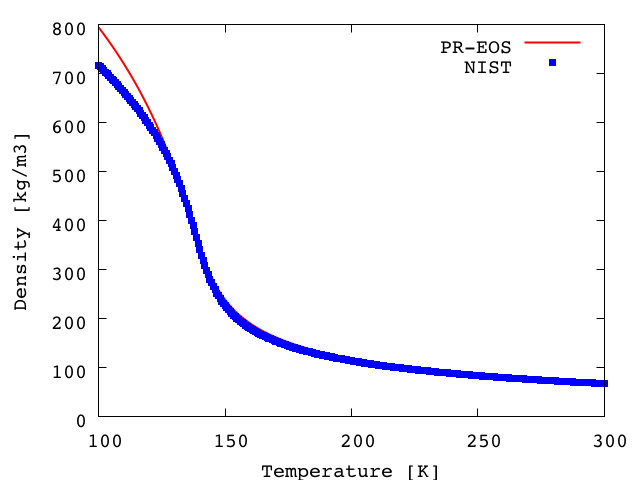
\includegraphics[height=1.8in]{figures/N2_vsNIST_Density.png}
        \caption{Density of nitrogen(N2) in [kg/$m^{3}$], as a function of Temperature at isobaric conditions, 60 bar}
    \end{subfigure}%
    ~ 
    \begin{subfigure}[t]{0.5\textwidth}
        \centering
        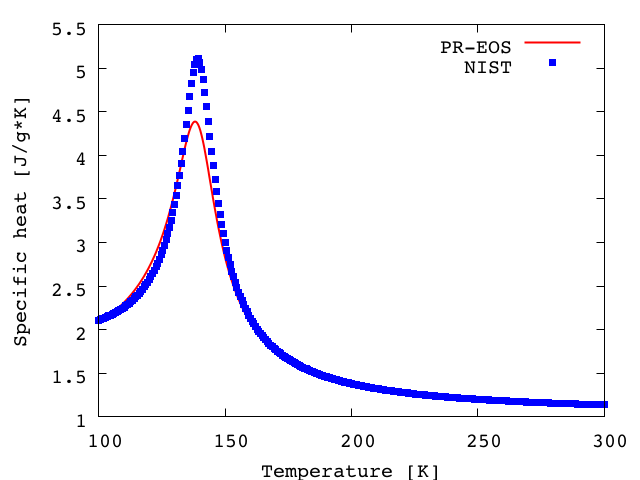
\includegraphics[height=1.8in]{figures/N2_vsNIST_Cp.png}
        \caption{Specific heat at constant pressure, Cp, of nitrogen(N2) in [J/g K], as a function of Temperature at isobaric conditions, 60 bar}
    \end{subfigure}
    \caption{Comparison of thermodynamic quantities (Density and Specific heat) computed using PR EOS against NIST}
    \label{fig:DensityCpVsNIST}
\end{figure}

\begin{figure}[t!]
    \centering
    \begin{subfigure}[t]{0.5\textwidth}
        \centering
        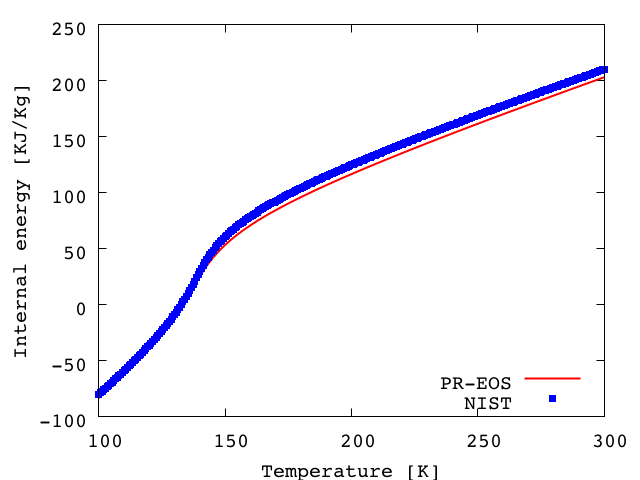
\includegraphics[height=1.8in]{figures/N2_vsNIST_InternalEnergy.png}
        \caption{Internal energy of nitrogen(N2) in [kJ/Kg], as a function of Temperature at isobaric conditions, 60 bar}
    \end{subfigure}%
    ~ 
    \begin{subfigure}[t]{0.5\textwidth}
        \centering
        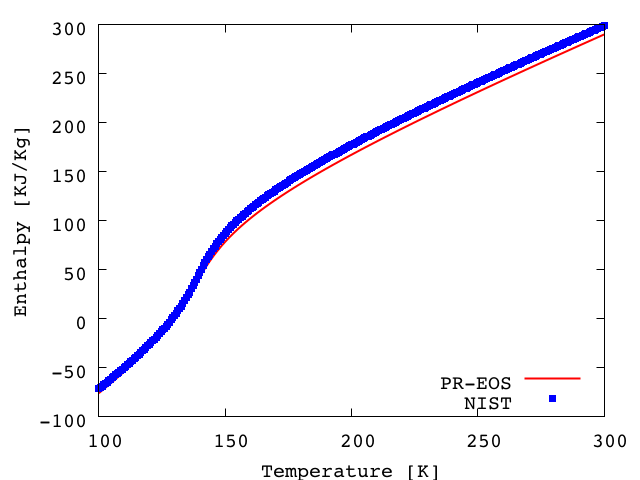
\includegraphics[height=1.8in]{figures/N2_vsNIST_Enthalpy.png}
        \caption{Enthalpy of nitrogen(N2) in [kJ/Kg], as a function of Temperature at isobaric conditions, 60 bar}
    \end{subfigure}
    \caption{Comparison of thermodynamic quantities (Internal energy and Enthalpy) computed using PR EOS against NIST}
    \label{fig:EnthalpyEnergyVsNIST}
\end{figure}

\cleardoublepage
\subsection{Conversion between state variables}
In order to test conversion between state variables, the data generated from PR-EOS presented in the previous section, Sec.~\ref{sec:ComparePRvsNIST} is relied upon. At first profiles of state variables, p, T, E and density, $\rho$
are generated at iso-baric conditions, p = 60 [bar] as a function of temperature.  
%\subsection{Computing density and Internal energy given Pressure and Temperature}     
%Given Pressure, $P_{in}$ and Temperature, $T_{in}$, the compressibility factor is computed using Eq.~\ref{eq:PReosCompressibility}. Thereafter, density, $\rho$ is computed using relation the $\rho = \frac{p M}{Z R_u T}$, where $M$ is the molecular weight. Using derivatives of EOS parameters, departure functions and thus internal energy can be computed using Eq.~\ref{eq:internalEnergyFinal}. 
%\begin{align}
%\rho_{p,T} & = F(P_{in},T_{in}) \\
%e_{p,T} & = E(P_{in},T_{in})
%\end{align}
%Plots comparing the data obtained from PR EOS against NIST are shown in Figs.~\ref{fig:DensityCpVsNIST}\&\ref{fig:EnthalpyEnergyVsNIST}. 
%\subsection{Computing Pressure and Internal energy given Density and Temperature}  
%Pressure, p, can be very easily expressed as a function of $\rho$ and T by arranging the terms of PR EOS, as shown in the equation below. 
%\begin{align}
%p &= \frac{\rho R_{m} T}{1-\rho b_m} - \frac{\rho^{2} a_m}{1 + 2 \rho b_m - \rho^2 b_m^{2}} \\
%a &= A_m/M^2 \\
%b &= B_m/M \\
%R_m &= R_u/M
%\label{eq:PreosPrho}
%\end{align}
%In order to test the implementation of this form of EOS, density,$\rho_{p,T}$, and Temperature, $T_{in}$, from the previous section are used to compute pressure, $p_{\rho, T}$. This pressure is then compared against $P_{in}$ in Fig.~\ref{fig:PfromRHOT}. Once the parameters in the EOS are set, various derivatives of EOS can be computed to generate internal energy, $e_{\rho, T}$ which is compared against $e_{p,T}$, in Fig.~\ref{fig:EfromRHOT}. 
%\begin{figure}[!tbh]
%    \centering
%    \begin{subfigure}[t]{0.5\textwidth}
%        \centering
%        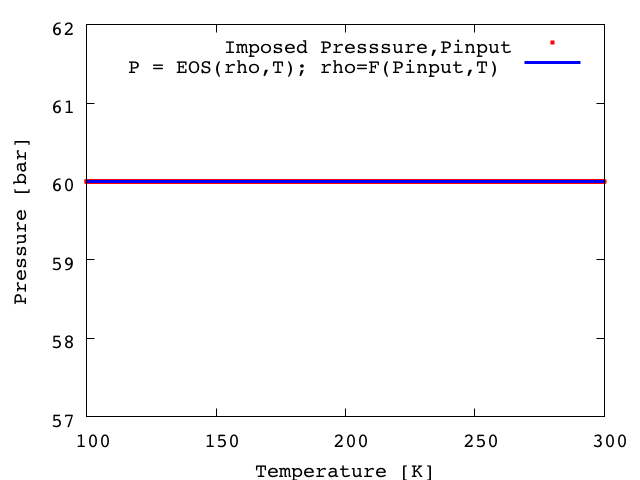
\includegraphics[height=1.8in]{figures/N2_NonLinear_PfromRHO_T.png}
%        \caption{Pressure of nitrogen(N2) in [bar], as a function of Temperature at isobaric conditions, 60 bar}
%        \label{fig:PfromRHOT}
%    \end{subfigure}%
%    ~ 
%    \begin{subfigure}[t]{0.5\textwidth}
%        \centering
%        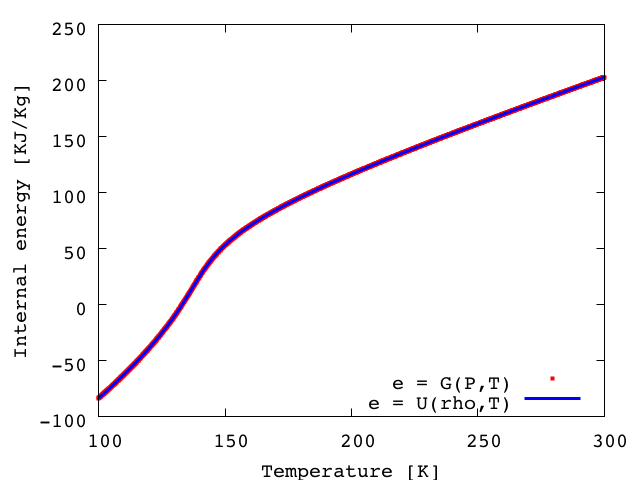
\includegraphics[height=1.8in]{figures/N2_NonLinear_EfromRHO_T.png}
%        \caption{Internal energy of nitrogen(N2) in [kJ/kg], as a function of Temperature at isobaric conditions, 60 bar}
%        \label{fig:EfromRHOT}
%    \end{subfigure}
%    \caption{Conversion between state variables, Pressure, P and Internal Energy, E computed from PR EOS, given Density, $\rho$ and Temperature}
%\end{figure}
\subsection{Computing Temperature and Internal energy given Pressure and density}  
As can be observed from Eq.~\ref{eq:PReosCompressibility}, compressibility factor, Z is a non-linear function of temperature, T. For this reason a non-linear root solve algorithm needs to be implemented to compute the root of the following function, F. 
\begin{align}
F &= ZT - \frac{P M}{\rho R_u} \\
G &= \frac{Z \rho R_u T}{M} - P 
\end{align}
where $\frac{P M}{\rho R_u}$ is known. This relationship can be recast as 
\begin{align}
G &= \frac{Z \rho R_u T}{M} - P 
\end{align}
This recasting allows us to easily calculate analytical derivative of G for implementation in a Newton-Raphson based root solve algorithm. The analytical derivative can be derived using Eq.~\ref{eq:PreosPrho} as following
\begin{align}
\frac{dG}{dT} = \left(\frac{\partial \rho}{\partial T} \right)_{\rho, X} = \frac{\rho R_m}{1-\rho b_m} - \frac{\rho^2 \frac{\partial a_m}{\partial T}}{1 + 2\rho b_m - \rho^2 b_m^{2}}
\end{align}
Using the ideal gas estimate of temperature as the initial guess, the Newton-Raphson based non-linear root solve algorithm converges to the expected solution,$T_{in}$. Fig.~\ref{fig:TEfromRHOP} shows the temperature comparison against $T_{in}$ and internal energy, $e_{P,\rho}$ against the internal energy, $e_{p,T}$ obtained using $P_{in}$ and Temperature, $T_{in}$. 
\begin{figure}[!tbh]
    \centering
    \begin{subfigure}[t]{0.5\textwidth}
        \centering
        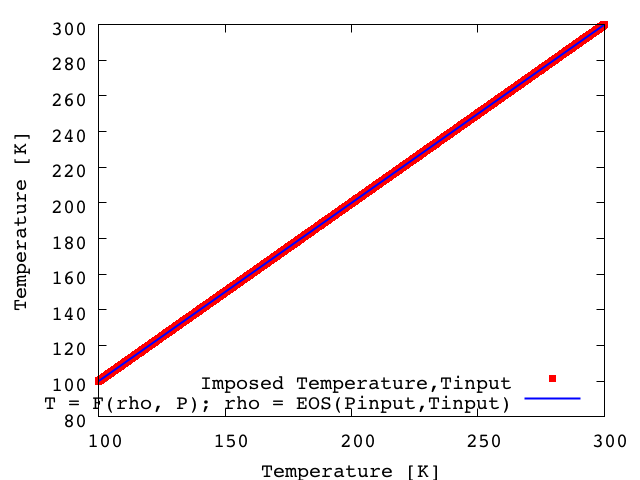
\includegraphics[height=1.8in]{figures/N2_NonLinear_TfromRHO_P.png}
        \caption{Temperature of nitrogen(N2) in [K]}
        \end{subfigure}%
    ~ 
    \begin{subfigure}[t]{0.5\textwidth}
        \centering
        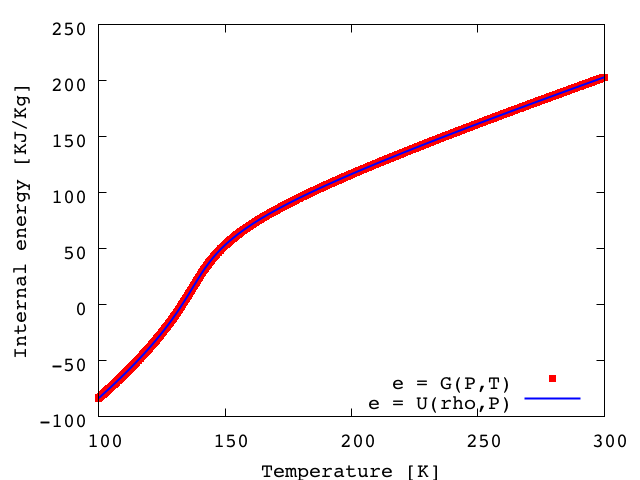
\includegraphics[height=1.8in]{figures/N2_NonLinear_EfromRHO_P.png}
        \caption{Internal energy of nitrogen(N2) in [kJ/kg], as a function of Temperature at isobaric conditions, 60 bar}
    \end{subfigure}
    \caption{Conversion between state variables, Temperature, T and Internal Energy, E computed from PR EOS, given Density, $\rho$ and Pressure}
    \label{fig:TEfromRHOP}
\end{figure}

\subsection{Computing Pressure and Temperature given Density and Internal energy}  
Since the Eq.~\ref{eq:internalEnergyFinal} is only a function of density and Temperature, a non-linear root solve algorithm to calculate temperature from density and internal energy is first employed. Thereafter, Pressure is computed using density and temperature. Using the following relations, a non-linear root solve based on Newton-Raphson algorithm can be constructed
\begin{align}
G\left( T \right) &= e^{*} - e^{ig}\left(T\right) - \left[ A_m(T) - T\frac{\partial A_m}{\partial T}\right]K_{1}\left(\rho^{*}\right) \\
\left(\frac{\partial G}{\partial T}\right)_{\rho} &= -C_v^{ig} + K_{1}\left(\rho^{*}\right) \left[T\frac{\partial^2 A_m}{\partial T^2} \right] 
\end{align}
where $e^{*}$ and $\rho^*$ are known quantities. 
\begin{figure}[!tbh]
    \centering
    \begin{subfigure}[t]{0.5\textwidth}
        \centering
        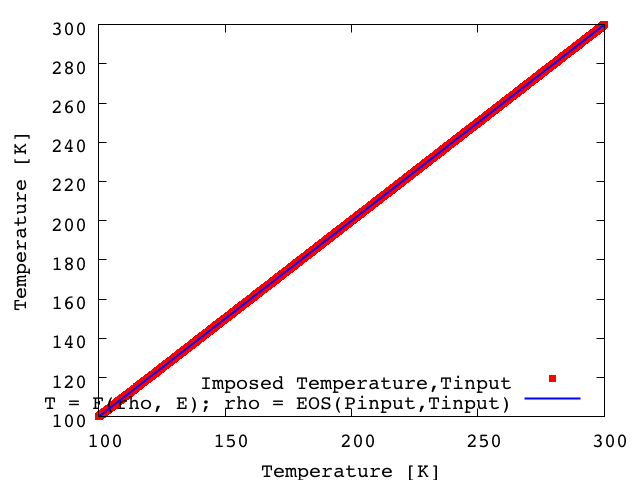
\includegraphics[height=1.8in]{figures/N2_NonLinear_TfromRHO_E.png}
        \caption{Temperature of nitrogen(N2) in [K]}
    \end{subfigure}%
    ~ 
    \begin{subfigure}[t]{0.5\textwidth}
        \centering
        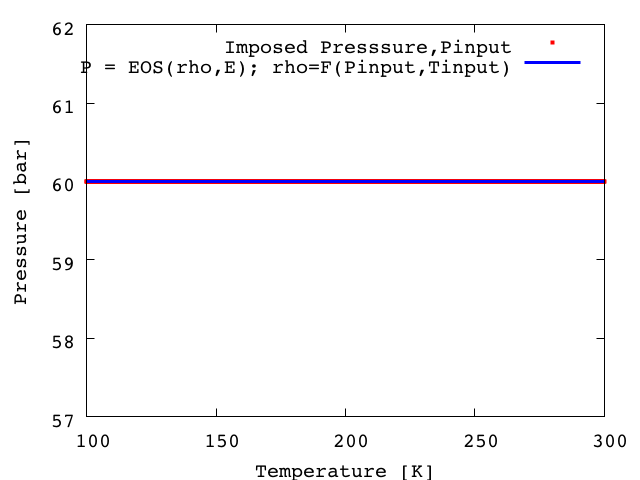
\includegraphics[height=1.8in]{figures/N2_NonLinear_PfromRHO_E.png}
        \caption{Pressure of nitrogen(N2) in [bar], as a function of Temperature at isobaric conditions, 60 bar}
    \end{subfigure}
    \caption{Conversion between various state variables, Temperature, T and Pressure, P computed from PR EOS, given Density, $\rho$ and Internal energy, E}
\end{figure}



\bibliographystyle{unsrt}% Produces the bibliography via BibTeX.
\bibliography{nonideal_refs}% Produces the bibliography via BibTeX.

\end{document}
